% !TEX TS-program = pdflatex
% !TEX encoding = UTF-8 Unicode

% This is a simple template for a LaTeX document using the "article" class.
% See "book", "report", "letter" for other types of document.

\documentclass[11pt]{article} % use larger type; default would be 10pt

\usepackage[utf8]{inputenc} % set input encoding (not needed with XeLaTeX)

%%% Examples of Article customizations
% These packages are optional, depending whether you want the features they provide.
% See the LaTeX Companion or other references for full information.

%%% PAGE DIMENSIONS
\usepackage{geometry} % to change the page dimensions
\geometry{a4paper} % or letterpaper (US) or a5paper or....
% \geometry{margin=2in} % for example, change the margins to 2 inches all round
% \geometry{landscape} % set up the page for landscape
%   read geometry.pdf for detailed page layout information

\usepackage{graphicx} % support the \includegraphics command and options

% \usepackage[parfill]{parskip} % Activate to begin paragraphs with an empty line rather than an indent

%%% PACKAGES
\usepackage{booktabs} % for much better looking tables
\usepackage{array} % for better arrays (eg matrices) in maths
\usepackage{paralist} % very flexible & customizable lists (eg. enumerate/itemize, etc.)
\usepackage{verbatim} % adds environment for commenting out blocks of text & for better verbatim
\usepackage{subfig} % make it possible to include more than one captioned figure/table in a single float
% These packages are all incorporated in the memoir class to one degree or another...

%%% HEADERS & FOOTERS
\usepackage{fancyhdr} % This should be set AFTER setting up the page geometry
\pagestyle{fancy} % options: empty , plain , fancy
\renewcommand{\headrulewidth}{0pt} % customise the layout...
\lhead{}\chead{}\rhead{}
\lfoot{}\cfoot{\thepage}\rfoot{}

%%% SECTION TITLE APPEARANCE
\usepackage{sectsty}
\allsectionsfont{\sffamily\mdseries\upshape} % (See the fntguide.pdf for font help)
% (This matches ConTeXt defaults)

%%% ToC (table of contents) APPEARANCE
\usepackage[nottoc,notlof,notlot]{tocbibind} % Put the bibliography in the ToC
\usepackage[titles,subfigure]{tocloft} % Alter the style of the Table of Contents
\renewcommand{\cftsecfont}{\rmfamily\mdseries\upshape}
\renewcommand{\cftsecpagefont}{\rmfamily\mdseries\upshape} % No bold!

% MATH
\usepackage{graphicx}

\usepackage{mathtools}
\usepackage{amsmath}
\usepackage{float}
\usepackage{listings}
%%% END Article customizations

%%% The "real" document content comes below...

\title{Numerical Optimization - Handin 6}
\author{Martin Simon Haugaard - CDL966}
%\date{} % Activate to display a given date or no date (if empty),
         % otherwise the current date is printed 

\begin{document}
\maketitle
\section{Programming}
This week it's all about implementing constraints in the Inverse Kinematics framework. I've chosen to stay with \textit{Steepest Descent} approch, and focus purely on implementing the constraints. My implementation works initially like any Steepest Descent method, by calculating a steepest descent direction
\begin{gather*}
p_k = -J'*(e-goal)
\end{gather*}
With Jacobian, $J$, desired location $goal$ and $e$ is the end-effector position.

Once the direction is computed, a desired location is computed by calculating a series of angles, which would best achieve the desired location. Figure~\ref{subfig:IK1} shows how this will look, when there are no constraints, or if the constraints applied are large enough not to have an effect (which is the case for this plot).
\begin{figure}[h!]
\subfloat[Unconstricted Steepest Descent Inverse Kinematic\label{subfig:IK1}]{%
      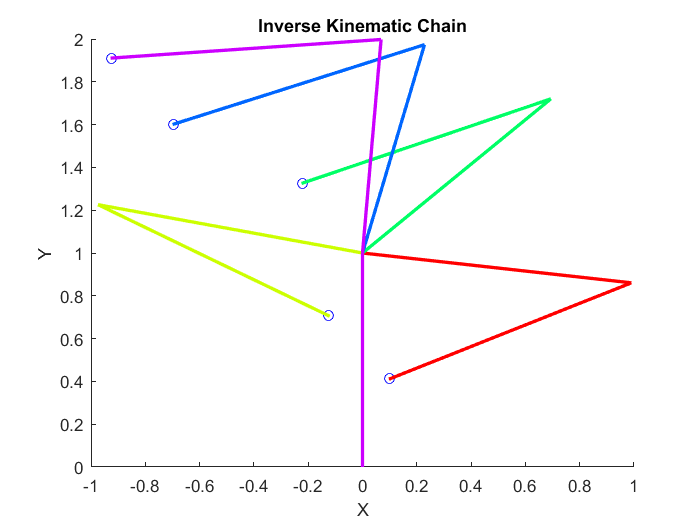
\includegraphics[width=0.45\textwidth]{IK}
    }
    \hfill
    \subfloat[Convergence Plot for Unconstricted Steepest Descent\label{subfig:convergence1}]{%
      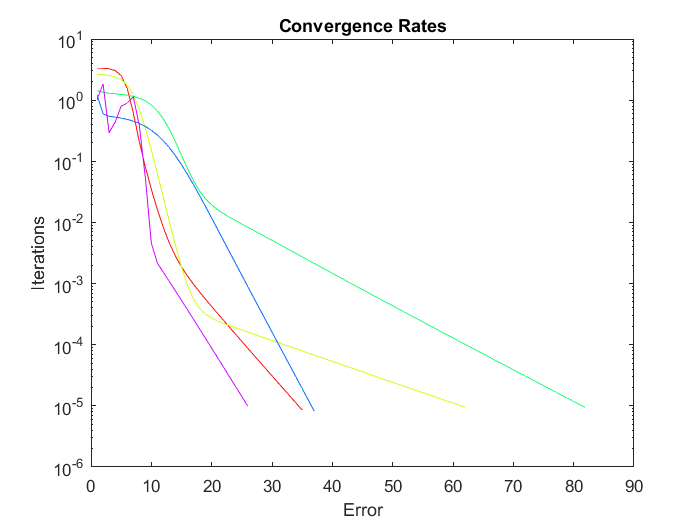
\includegraphics[width=0.45\textwidth]{convergence}
    }
\caption{}
\label{fig:IK1}
\end{figure}
To verify that the steepest descent is in effect, the convergence plot is seen in Figure~\ref{subfig:convergence1}. It can be seen that the convergence plot error
\begin{gather*}
    error      = 0.5*||r||^2
\end{gather*}
where $r = e-goal$, is almost logaritmic, which is the desired effect we want.

To add the constraints an alteration was made to the Line Search algorithm in use. After calculating the ideal angles, these are sent through a projection script, which will make sure they are all within the given constraints, as described in (16.69).  Because of the constraints, an alteration is needed on the Backtracking Line Search algorithm (P. 37).

Instead of the original:
\begin{gather*}
\text{While} ~ f(x_k) + c \alpha \nabla f_k^T p_k <=f(x_k + \alpha p_k) \{ \dots \}
\end{gather*}

A loop taking the projecting into account is needed:
%while (f + c*gradF'*dif <= f_new & iter < max_iter)    
\begin{gather*}
\text{While} ~ error_{projected} + c \alpha \nabla f_k * (\theta_{projected} -\theta_{org}) <= error_{org}
\end{gather*}
This loop guarentees that the projected angles are still approching the desired location, but allows the new angles to be projections.

\begin{figure}[h!]
\subfloat[Constricted Steepest Descent Inverse Kinematic\label{subfig-1:dummy}]{%
      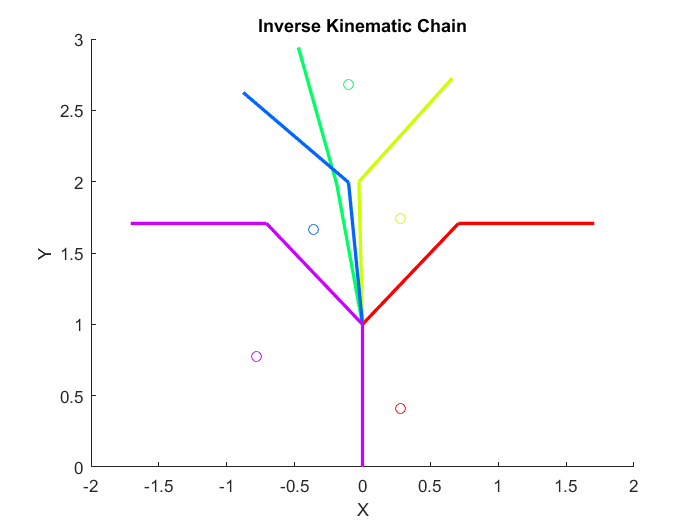
\includegraphics[width=0.45\textwidth]{IK-reduced-angle}
    }
    \hfill
    \subfloat[Convergence Plot for constricted Steepest Descent\label{subfig-2:dummy}]{%
      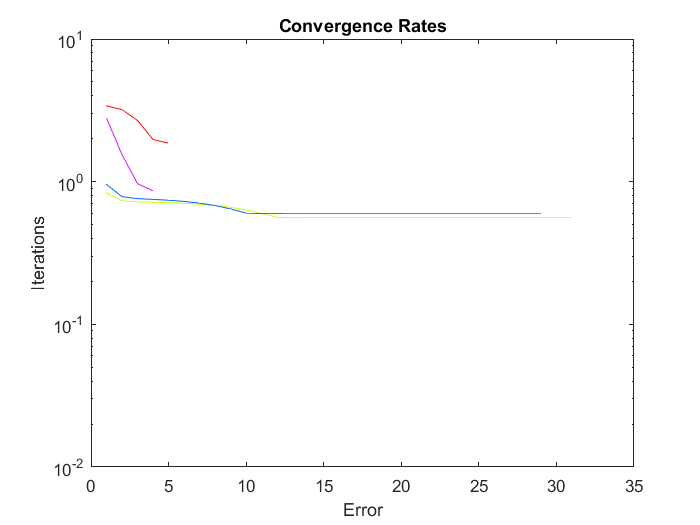
\includegraphics[width=0.45\textwidth]{convergence-reduced-angle}
    }
\caption{}
\label{fig:IK2}
\end{figure}
In Figure~\ref{fig:IK2} the constraining angle were set to $\frac{\pi}{4}$ and $-\frac{\pi}{4}$ for all the joints. This allows for a 90 degree angle in total in which the joints can move. Observing the red and purple plots, the angle between these is indeed 90 degrees. And for both of these examples they all their angles are at the maximum allowed angle for each of the joints, just in opposite directions. The convergence plots for these are almost linear when plotted on a logaritmic scale, however, the error is generally a lot bigger. Which makes sense since we are adding limits as to how close to the ideal we allow it to be.

As for the rest of the three plots, they struggle a bit more trying to approch the minimum. As seen by the increased number of iterations conducted, however, they do manage to make what seems to be the best possible approximation, given the constraints.

A general flaw I found when using Steepest Descent, was the dependencies on the initial guess. When trying to reach a point, outside the reachable area, depending on the initial guess, the approximation may be fairly good, or horribly wrong.

\begin{figure}[h!]
\subfloat[Constricted Steepest Descent Inverse Kinematic\label{guess_IK}]{%
      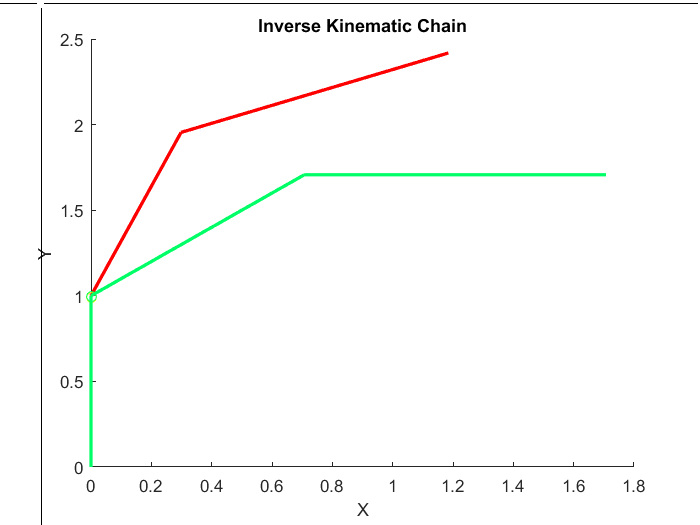
\includegraphics[width=0.45\textwidth]{initial_0}
    }
    \hfill
    \subfloat[Convergence Plot for constricted Steepest Descent\label{guess_convergence}]{%
      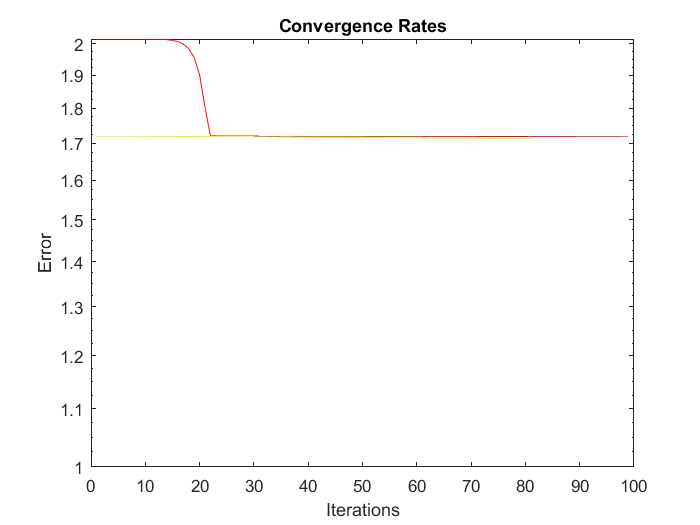
\includegraphics[width=0.45\textwidth]{initial}
    }
\caption{}
\label{fig:IK2}
\end{figure}
Figure~\ref{guess_IK} shows two plots, both with the desired location \begin{math}x^*=\begin{pmatrix}0\\1\end{pmatrix}\end{math}. The Green plot has initial angles $[0;0;0]$ while the red plot reuses the green plot's end final angles. It can be seen two different results are given. The cause likely being that Steepest Descent lacks the smarts to realize that it's already in an ideal position when starting, and it naively tries to improve upon the initial guess. It's a general error I tend to have, I can't, at the moment, find a good way of making the initial angles, without having a few of my results clearly being affected by poor start location.
\section{Exercises}
\section*{12.13}
\begin{gather*}
(x_1 - 1)^2 + (x_2 -1)^2 \leq 2,\\
(x_1 -1)^2 + (x_2 +1)^2 \leq 2,\\
x_1 \geq 0
\end{gather*}
is the same as writing constraints
\begin{gather*}
c_1(x) = 2 - (x_1-1)^2-(x_2-1)^2\geq 0,\\
c_2(x)=2-(x_1-1)^2-(x_2+1)^2\geq 0,\\
c_3(x)=x_1 \geq 0
\end{gather*}
Giving
\begin{gather*}
\nabla c_1(x) = \begin{bmatrix}-2(x_1 -1) \\ -2(x_2 -1)\end{bmatrix}\\
\nabla c_2(x) = \begin{bmatrix}-2(x_1 -1) \\ -2(x_2 +1)\end{bmatrix}\\
\nabla c_3(x) = \begin{bmatrix}1\\0\end{bmatrix}
\end{gather*}
All the sets are active in \begin{math}x^* = (0,0)^T\end{math} meaning the dimensions of the problem is 3. However, the dimensions of the problem is limited to 2. For LICQ to be linear independent
\begin{gather*}
\nabla c_1(x), i\in A(x)
\end{gather*}
Which is not the case, hence LICQ is not satisfied.

For MFCQ, there has to be a vector \begin{math}w\in R^n \text{ such that } \nabla c_1(x^*)^T w > 0 \text{ for all } i \in A(x^*) \cap  I\end{math}, this however does hold (\begin{math}w=(1,0)\end{math}). Thus MFCQ is satisfied.
\end{document}
